\documentclass[main.tex]{subfiles}
\begin{document}
\subsection{Show that the 36 matrices $\sigma_a\otimes\mathbb{I}\otimes\mathbb{I}\equiv\sigma_a$, $\mathbb{I}\otimes\tau_a\otimes\mathbb{I}\equiv\tau_a$, $\mathbb{I}\otimes\mathbb{I}\otimes\eta_a\equiv\eta_a$, $\sigma_a\otimes\tau_b\otimes\eta_c\equiv\sigma_a\tau_b\eta_c$ form a Lie algebra. Find the roots, simple roots and the Dynkin diagram. What is the algebra?}
First, construct the commutators
\begin{align}
[\sigma_a,\sigma_b]=&2\img\epsilon_{abc}\sigma_c\\
[\tau_a,\tau_b]=&2\img\epsilon_{abc}\tau_c\\
[\eta_a,\eta_b]=&2\img\epsilon_{abc}\eta_c\\
[\sigma_a,\tau_b]=&[\sigma_a,\eta_b]=[\tau_a,\eta_b]=0\\
[\sigma_a,\sigma_b\tau_c\eta_d]=&2\img\epsilon_{abe}\sigma_e\tau_b\eta_c\\
[\tau_a,\sigma_b\tau_c\eta_d]=&2\img\epsilon_{ace}\sigma_a\tau_e\eta_c\\
[\sigma_a,\sigma_b\tau_c\eta_d]=&2\img\epsilon_{ace}\sigma_a\tau_b\eta_e\\
[\sigma_a\tau_b\eta_c,\sigma_d\tau_e\eta_f]=&\sigma_a\sigma_d\otimes(\delta_{be}\delta_{cf}\mathbb{I}\otimes\mathbb{I}+\img\epsilon_{bei}\delta_{cf}\tau_i\otimes\mathbb{I}+\img\epsilon_{cfi}\delta_{be}\mathbb{I}\otimes\eta_i-\epsilon_{bei}\epsilon_{cfj}\tau_i\otimes\eta_j)\nonumber\\
&-\sigma_d\sigma_a\otimes(\delta_{be}\delta_{cf}\mathbb{I}\otimes\mathbb{I}-\img\epsilon_{bei}\delta_{cf}\tau_i\otimes\mathbb{I}-\img\epsilon_{cfi}\delta_{be}\mathbb{I}\otimes\eta_i-\epsilon_{bei}\epsilon_{cfj}\tau_i\otimes\eta_j)\\
=&2\img\epsilon_{adi}\delta_{be}\delta_{cf}\sigma_i\otimes\mathbb{I}\otimes\mathbb{I}+2\img\epsilon_{bei}\delta_{cf}\delta_{ad}\mathbb{I}\otimes\tau_{i}\otimes\mathbb{I}+2\img\epsilon_{cfi}\delta_{be}\delta_{ad}\mathbb{I}\otimes\mathbb{I}\otimes\eta_i\nonumber\\
&-2\img\epsilon_{adk}\epsilon_{bei}\epsilon_{cfj}\sigma_k\otimes\tau_i\otimes\eta_j\\
=&2\img\left(\epsilon_{adi}\delta_{be}\delta_{cf}\sigma_i  + \epsilon_{bei}\delta_{cf}\delta_{ad}\tau_{i} +  \epsilon_{cfi}\delta_{be}\delta_{ad}\eta_i -\epsilon_{adk}\epsilon_{bei}\epsilon_{cfj}\sigma_k\tau_i\eta_j  \right).
\end{align}
Thus the commutators close and the matrices form a Lie algebra.

We pick the Cartan subalgebra as
\begin{align}\label{eq:19ACartan}
H_1=\sigma_3=&\text{diag}\begin{pmatrix}1,&1,&1,&1,&-1,&-1,&-1,&-1,\end{pmatrix}\\
H_2=\tau_3=&\text{diag}\begin{pmatrix}1,&1,&-1,&-1,&1,&1,&-1,&-1\end{pmatrix}\\
H_3=\eta_3=&\text{diag}\begin{pmatrix}1,&-1,&1,&-1,&1,&-1,&1,&-1\end{pmatrix}\\
H_4=\sigma_3\tau_3\eta_3=&\text{diag}\begin{pmatrix}1,&-1,&-1,&1,&-1,&1,&1,&-1\end{pmatrix}.
\end{align}
The $H_m$ all have eigenvalues $\lambda=\pm1$ and the eigenvectors are given by the eight dimensional unit vectors which we may write in component form as $[e^k]_m=\delta^k_m$, $k,m=1...8$ e.g.
\begin{equation}
e^2=\begin{pmatrix}0\\1\\0\\0\\0\\0\\0\\0\end{pmatrix}.
\end{equation}
Then, the weights are given by
\begin{align}
\mu_1&=(1,1,1,1)=-\mu_8\\
\mu_2&=(1,1,-1,-1)=-\mu_7\\
\mu_3&=(1,-1,1,-1)=-\mu_6\\
\mu_4&=(1,-1,-1,1)=-\mu_5.
\end{align}
Then we expect $36-4=32$ roots for the $32$ remaining generators. We can construct $4\cdot3\cdot2=24$ of the roots by considering just $\mu_k$ for $k=1..4$, since $\mu_1=-\mu_8$, etc. The generators connect the weight vectors so that 24 of the roots are given by the difference in the weights $\pm\mu_i\pm\mu_j$, $i,j=1..4$, $i\neq j$. The remaining $8$ roots must just be the weights themselves $\pm\mu_i$, $i=1...4$.

Defining positivity to be from left to right the normalised simple roots are given by the lowest positive state
\begin{align}
\alpha_1&=\mu_1-\mu_2=\frac{1}{\sqrt{8}}(0,0,2,2)\\
\alpha_2&=\mu_2-\mu_3=\frac{1}{\sqrt{8}}(0,2,-2,0)\\
\alpha_3&=\mu_3-\mu_4=\frac{1}{\sqrt{8}}(0,0,2,-2)\\
\alpha_4&=\mu_4=\frac{1}{2}(1,-1,-1,1).
\end{align}
To obtain the Dynkin diagram we use the formula $\theta_{\alpha_i\alpha_j}=\arccos{\left(\frac{\alpha_i\cdot\alpha_j}{\sqrt{\alpha_i^2\alpha_j^2}}\right)}$. So that
\begin{align}
\theta_{\alpha_1\alpha_2}&=\frac{2}{3}\pi\\
\theta_{\alpha_2\alpha_3}&=\frac{2}{3}\pi\\
\theta_{\alpha_3\alpha_4}&=\frac{3}{4}\pi
\end{align}
So the Dynkin diagram is 
\begin{figure}[H] 
\centering
  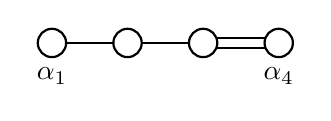
\begin{tikzpicture}[scale=.6]
    \draw[thick] (-1.6,0) circle (.3);
    \draw[thick] (-0.3, 0 ) -- +(-1 ,0);
    \draw[thick] (0,0) circle (.3);
    \draw[thick] (0.3, 0 ) -- +(1 ,0);
    \draw[thick] (1.6,0) circle (.3);
    \draw[thick] (1.9, 0.1 ) -- +(1 ,0);
    \draw[thick] (1.9, -0.1 ) -- +(1 ,0);
    \draw[thick] (3.2,0) circle (.3);
    \node at (-1.6,-0.7) {$\alpha_1$};
    \node at (3.2,-0.7) {$\alpha_4$};
  \end{tikzpicture}
\end{figure}
which is $B_4$ or $\mathfrak{so}(9)$.

\subsection{Show that the 28 matrices $\sigma_a\otimes\mathbb{I}\otimes\mathbb{I}\equiv\sigma_a$, $\mathbb{I}\otimes\tau_a\otimes\mathbb{I}\equiv\tau_a$, $\mathbb{I}\otimes\mathbb{I}\otimes\eta_3\equiv\eta_3$, $\sigma_a\otimes\eta_1\otimes\mathbb{I}\equiv\sigma_a\eta_1$, $\sigma_a\otimes\eta_2\otimes\mathbb{I}\equiv\sigma_a\eta_2$, $\mathbb{I}\otimes\tau_a\otimes\eta_1\equiv\tau_a\eta_1$, $\mathbb{I}\otimes\tau_a\otimes\eta_2\equiv\tau_a\eta_2$, $\sigma_a\otimes\tau_b\otimes\eta_3\equiv\sigma_a\tau_b\eta_3$ form a Lie algebra. Find the roots, simple roots and the Dynkin diagram. What is the algebra?}
To show the matrices form a Lie algebra we can, rather long-windedly, evaluate the commutators, letting Greek indices $\mu,\nu$ run from $1$ to $2$,
\begin{align}
[\sigma_a,\sigma_b]=&2\img\epsilon_{abc}\sigma_c\\
[\sigma_a,\sigma_b\eta_{\mu}]=&2\img\epsilon_{abc}\sigma_c\eta_{\mu}\\
[\sigma_a,\tau_{\mu}]=&[\sigma_a,\tau_b\eta_{\mu}]=0\\
[\sigma_a,\sigma_b\tau_c\eta_3]=&2\img\epsilon_{abd}\sigma_d\tau_c\eta_3\\
[\tau_a,\tau_b]=&2\img\epsilon_{abc}\tau_c\\
[\tau_a,\tau_b\eta_{\mu}]=&2\img\epsilon_{abc}\tau_c\eta_{\mu}\\
[\tau_a,\sigma_b\tau_c\eta_3]=&2\img\epsilon_{acd}\sigma_b\tau_d\eta_3\\
[\tau_a,\eta_3]=&[\tau_a,\sigma_b\eta_{\mu}]=0\\
[\eta_3,\eta_3]=&[\eta_3,\sigma_a\tau_b\eta_3]=0\\
[\eta_3,\sigma_a\eta_{\mu}]=&2\img\epsilon_{3\mu\nu}\sigma_a\eta_{\nu}\\
[\eta_3,\tau_a\eta_{\mu}]=&2\img\tau_a\eta_{\mu}\\
[\sigma_a\eta_{\nu},\sigma_b\eta_{\mu}]=&2\img\epsilon_{abc}\sigma_c(\delta_{\nu\mu}\mathbb{I}+\img\epsilon_{\mu\nu3}\eta_3)\\
[\sigma_a\eta_{\mu},\tau_b\eta_{\nu}]=&2\img\epsilon_{\mu\nu3}\sigma_a\tau_b\eta_3=0\\
[\sigma_a\eta_{\mu},\sigma_b\tau_c\eta_3]=&2\epsilon_{abd}\sigma_d\tau_c(\delta_{\nu\mu}\mathbb{I}+\img\epsilon_{\mu\nu3}\eta_3)\\
[\tau_a\eta_{\mu},\tau_b\eta_{\nu}]=&2\img\epsilon_{abc}\tau_c(\delta_{\nu\mu}\mathbb{I}+\img\epsilon_{\mu\nu3}\eta_3)\\
[\sigma_a\tau_b\eta_3,\sigma_c\tau_d\eta_3]&=2\img\epsilon_{ace}\delta_{bd}\sigma_e+2\img\epsilon_{bde}\delta_{ac}\tau_e.
\end{align}
 and thus the algebra closes under commutation so the matrices form a Lie algebra.
 
The algebra is also of rank 4, and we may pick the Cartan generators to be the same as those in Problem(19.A) given by \eqref{eq:19ACartan}, therefore the weight are the same also, the difference now is that we have only $28-4=24$ roots given by $\pm\mu_i\pm\mu_j$, $i\neq j$, $i,j=1...4$, now the normalised simple roots are just
\begin{align}
\alpha_1&=\mu_1-\mu_2=\frac{1}{\sqrt{8}}(0,0,2,2)\\
\alpha_2&=\mu_2-\mu_3=\frac{1}{\sqrt{8}}(0,2,-2,0)\\
\alpha_3&=\mu_3-\mu_4=\frac{1}{\sqrt{8}}(0,0,2,-2)\\
\alpha_4&=\mu_3+\mu_4=\frac{1}{\sqrt{8}}(2,-2,0,0).
\end{align}
with the angles between the simple roots given by
\begin{align}
\theta_{\alpha_1\alpha_2}&=\frac{2}{3}\pi\\
\theta_{\alpha_2\alpha_3}&=\frac{2}{3}\pi\\
\theta_{\alpha_2\alpha_4}&=\frac{2}{3}\pi
\end{align}
and the Dynkin diagram is therefore
\begin{figure}[H] 
\centering
  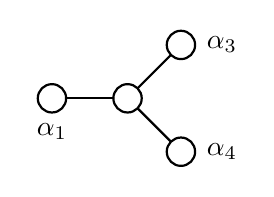
\begin{tikzpicture}[scale=.6]
    \draw[thick] (0,0) circle (.3);
    \draw[thick] (0.3, 0 ) -- +(1 ,0);
    \draw[thick] (1.6,0) circle (.3);
    \draw[thick] (1.81, 0.21 ) -- +(0.707 ,0.707);
    \draw[thick] (2.73,1.13) circle (.3);
    \draw[thick] (1.81, -0.21 ) -- +(0.707 ,-0.707);
    \draw[thick] (2.73,-1.13) circle (.3);
    \node at (0,-0.7) {$\alpha_1$};
    \node at (3.6,1.13) {$\alpha_3$};
    \node at (3.6,-1.13) {$\alpha_4$};
  \end{tikzpicture}
\end{figure}
Which is $D_4$ or $\mathfrak{so}(8)$.
\end{document}